\documentclass[10pt]{article}
\usepackage[en]{prettytex/base}
\usepackage{prettytex/math}
\usepackage{prettytex/code}
\usepackage{prettytex/contract}
\usepackage[toc, acronym, style=long3col, indexonlyfirst=true, nogroupskip=true]{glossaries}
\usepackage[backend=biber, citestyle=authoryear, bibstyle=authoryear, hyperref=true, sorting=none, maxbibnames=99]{biblatex}
\usepackage{csquotes}
\usepackage[nameinlink]{cleveref}
\usepackage{dsfont}
\usepackage{siunitx}

% Reporting
% from: https://static.uni-graz.at/fileadmin/projekte/biotechmedgraz/Programme/Lab_Rotation/Lab_Rotation_Program_Guidelines_2023.pdf
% The LRP awardee will be required to submit a short final report about his/her scientific activities during
% the rotation. The report must be signed by the lab rotation mentor.
% Report details: Max. 6 pages, composed of:
% • Summary
% • Introduction
% • Methods
% • Results
% • Future perspectives
% Reports must be submitted at the end of the fourth month of the lab rotation. The approval of the
% report is the basis for the transferal of the second instalment of the stipend.

% Was ist beim Endbericht zu beachten?
% from: https://biotechmedgraz.at/de/mitgliederbereich/programme/fragen-und-antworten-zum-biotechmed-graz-lab-rotation-programm/
% Der von Ihrem/Ihrer Betreuer*in unterzeichnete Endbericht ist spätestens am letzten Tag Ihrer Lab Rotation per E-Mail an die BioTechMed-Graz Geschäftsstelle zu senden. Bitte beachten Sie Details zum Endbericht in den Lab Rotation Richtlinien.

% https://physics.stackexchange.com/questions/302553/deriving-biot-savart-law-from-maxwells-equations

\title{Magnetic Resonance Current Density Imaging}
\author{Peter Julius Waldert}
\date{29\th of February, 2024}

\makenoidxglossaries
\newacronym{mri}{MRI}{Magnetic Resonance Imaging}
\newacronym{mrt}{MRT}{Magnetic Resonance Tomography}
\newacronym{mrcdi}{MRCDI}{Magnetic Resonance Current Density Imaging}
\newacronym{fft}{FFT}{Fast Fourier Transform}
\newacronym{ifft}{IFFT}{Inverse Fast Fourier Transform}
\newacronym{cdi}{CDI}{Current Density Imaging}
\newacronym{tv}{TV}{Total Variation}

\addbibresource{../literature/sources.bib}

\renewcommand{\norm}[1]{\left\lVert#1\right\rVert_{\scriptscriptstyle 2}}

\begin{document}
  \makeatletter
  \begin{center}
    {\Huge \@title} \\
    a\hspace{.4em}{\large BioTechMed-Graz Lab Rotation Report}
    \vspace{.5cm}

    of\hspace{.5em}{\large \@author}
    \vspace{.3cm}

    supervised by \textbf{Prof. Kristian Bredies} at the \\
    Institute of Mathematics and Scientific Computing (IMSC), \\
    University of Graz, Austria,
    \vspace{.3cm}

    {\@date}.
  \end{center}
  \makeatother

  \section{Summary}
  This lab rotation project was concerned with the development, exploration and implementation of a new optimisation approach for the reconstruction of current density / conductivity of tissue within a \gls{mri} setup.

  The project was split into two steps: First, simulating the magnetic field modulation given a current density field inside a \textit{phantom} (the \textit{forward} procedure), cf. \Cref{sec:fft-biot}.
  And second, reconstructing current density (including conductivity) using a novel optimisation model, based on measurements of the z-component of the magnetic field, with insight gained from the forward procedure (which, in turn is referred to as the \textit{backward} procedure), cf. \Cref{sec:optimisation-procedure}.

  The implementation was built on top of KomaMRI \parencite{2022-koma-mri} and is freely available on GitHub (\url{https://github.com/MrP01/CurrentDensityImaging}).
  An exemplary reconstruction is documented in the results (\Cref{sec:results}).

  \section{Introduction}
  The overall intention of \gls{mri} is to turn a source of contrast into an image for clinicians to use, mainly for the identification of different (potentially malignant) tissue types.
  In the usual setting, this source of contrast is one of the $T_1$, $T_2$ or $T_2^*$ material constants.
  Visualising these material properties in an image therefore allows to differentiate between different types of tissue visually.

  \subsection{Brief Introduction to Magnetic Resonance Imaging}
  What we image specifically are magnetic dipoles, also referred to as \textit{spins} in this context.
  The general equation governing the behaviour of these \textit{spin} objects is the Bloch equation:
  \begin{equation}
    \frac{\dd \vec{M}}{\ddt} = \gamma (\vec{M} \times \vec{B}) - \frac{(M_z - M_0) \vec{e_z}}{T_1} - \frac{M_x \vec{e_x} + M_y \vec{e_y}}{T_2}\,,
    \label{eq:bloch}
  \end{equation}
  where $\vec{M} = (M_x, M_y, M_z)^T \in \R^3$ is the magnetisation, $\vec{B} \in \R^3$ the magnetic field, $M_0 \in \R$ the equilibrium magnetisation, $T_1$ and $T_2 \in \R$ the (\textit{relaxation time}) material constants mentioned above and $t \in \R$ being time.

  Starting from a certain \gls{mri} sequence controlling the gradient coils to excite spins inside the object of interest (individually governed by \Cref{eq:bloch}), the imaging process generally travels through a grid of points in $\vec{k}$-space (Fourier space) to later reconstruct an image slice from the inverse Fourier transform.
  This procedure is repeated for every slice of the object until a full image is reconstructed (details may be found in \cite{1996-mri-basics}).

  For the purposes of \gls{mrcdi}, the procedure also yields the z-component of the magnetic field $B_z = B_3 = \{\vec{B}\}_3$, which we will use for the reconstruction of current density.

  \subsection{The Biot-Savart Law}
  For a given current density $\vec{j}(t): \Omega \to \R^3$ \footnote{
    The current density $\vec{j} = nq\vec{v}$, describing the flow of $n$ charges $q$ with velocity $\vec{v}$, may be related to \textit{current} $I$ through the infinitesimal $\vec{j} \idd^3\vec{x} = I \idd\vec{x}$.
  } on a domain $\Omega \subseteq \R^3$ at time $t \in \R^+$, Maxwell's fourth equation in differential form
  \begin{equation*}
    \nabla \times \vec{B} = \mu_0 \left(\vec{j} + \epsilon_0 \frac{\partial \vec{E}}{\partial t}\right)\,,
    \label{eq:maxwell-4}
  \end{equation*}
  relates the curl of the magnetic field $\vec{B}(t): \Omega \to \R^3$ to the current density $\vec{j}(t)$ and the temporal rate of change in the \textit{electric} field $\vec{E}(t): \Omega \to \R^3$.
  $\epsilon_0$ and $\mu_0$ are the electric permittivity and magnetic permeability of free space, respectively.
  The current density $\vec{j}$ is also connected to the electric field $\vec{E}$ through the, also position-dependent, electrical conductivity $\sigma: \Omega \to \R^+$
  $$\vec{j} = \sigma \vec{E}\,.$$

  In the \textbf{electrostatic case} (when the electric field $\vec{E}$ is indepent of time $t$), the last term in the above equation will vanish and we arrive at
  \begin{equation}
    \nabla \times \vec{B} = \mu_0 \vec{j}\,.
    \label{eq:maxwell-4-electrostatic}
  \end{equation}
  This equation, together with the freedom of divergence of the magnetic field (Maxwell's second equation), $\nabla \cdot \vec{B} = 0$, leads to the \textbf{Biot-Savart law}
  \begin{equation}
    \vec{B}(\vec{x})
    = \frac{\mu_0}{4\pi} \int_\Omega \frac{\vec{j}(\vec{y}) \times (\vec{x} - \vec{y})}{\norm{\vec{x} - \vec{y}}^3} \idd\vec{y}
    = \frac{\mu_0}{4\pi} \int_\Omega \frac{\vec{j}(\vec{y}) \times \vec{y}}{\norm{\vec{y}}^3} \idd\vec{y}
    \label{eq:biot-savart}
  \end{equation}
  which provides an explicit expression for the magnetic field contribution $\vec{B}(\vec{x})$ at position $\vec{x} \in \Omega$ given a current density field $\vec{j}$.

  \subsection{Current Density Imaging}
  Using a current source and attaching it to two electrodes connected to the object of interest, while reconstructing the image inside the \gls{mrt} tube, the \textit{imaging current} will induce a magnetic field modulation on top of the magnetic field inside the tube according to the Biot-Savart law, which we can measure (the $B_z$ component), cf. \cite{2004-mrcdi-from-one-var}.

  As we only have access to one component of the magnetic field, the resulting system is underdetermined and we therefore need to solve an \textit{inverse problem}.

  \section{Methods}
  For visualisation and as a general framework, we built upon the \textbf{KomaMRI} toolchain and Julia software package \parencite{2022-koma-mri}.
  This choice was made mostly due to Koma's feature-richness and extensibility, while harnessing the computational power of Julia \parencite{2017-julia}.

  \subsection{FFT-accelerated evaluation of the Biot-Savart law}
  \label{sec:fft-biot}
  Starting from the Biot-Savart law introduced above (cf. \Cref{eq:biot-savart}), we observe that splitting the cross-product ($\times$) into its three respective components
  \begin{align*}
    B_1(\vec{x}) & = \frac{\mu_0}{4\pi} \int_{\Omega} \frac{j_2(\vec{y}) \cdot (x_3 - y_3) - j_3(\vec{y}) \cdot (x_2 - y_2)}{\norm{\vec{x} - \vec{y}}^3} \idd\vec{y} \,, \\
    B_2(\vec{x}) & = \frac{\mu_0}{4\pi} \int_{\Omega} \frac{j_3(\vec{y}) \cdot (x_1 - y_1) - j_1(\vec{y}) \cdot (x_3 - y_3)}{\norm{\vec{x} - \vec{y}}^3} \idd\vec{y} \,, \\
    B_3(\vec{x}) & = \frac{\mu_0}{4\pi} \int_{\Omega} \frac{j_1(\vec{y}) \cdot (x_2 - y_2) - j_2(\vec{y}) \cdot (x_1 - y_1)}{\norm{\vec{x} - \vec{y}}^3} \idd\vec{y} \,,
  \end{align*}
  according to the explicit representation of the cross-product $\times$ in three spatial dimensions, most notably allows us to express $B_1$, $B_2$ and $B_3$ as convolution integrals
  $$B_1(\vec{x}) = \frac{\mu_0}{4\pi} \int_{\Omega} \big[j_2(\vec{y}) g_3(\vec{x} - \vec{y}) - j_3(\vec{y}) g_2(\vec{x} - \vec{y})\big]\idd\vec{y} = \frac{\mu_0}{4\pi} \big[(j_2 *_{\Omega} g_3) - (j_3 *_{\Omega} g_2)\big](\vec{x})\,,$$
  with $g_1, g_2, g_3: \Omega \to \R$, $g_1(\vec{x}) = \frac{\vec{x}_1}{\norm{\vec{x}}^3}$, $g_2(\vec{x}) = \frac{\vec{x}_2}{\norm{\vec{x}}^3}$ and $g_3(\vec{x}) = \frac{\vec{x}_3}{\norm{\vec{x}}^3}$ and the respective analogs for $B_2$ and $B_3$ \parencite{2020-biot-savart-evaluation-fft}.

  Using the convolution theorem for two functions $f$ and $g$
  $$\mathcal{F}[f * g](\vec{k}) = \mathcal{F}[f](\vec{k}) \cdot \mathcal{F}[g](\vec{k}) \quad\text{where}\quad \mathcal{F}[f](\vec{k}) := \int f(\vec{x}) \e^{-\i \vec{k} \vec{x}}\idd\vec{x}\,,$$
  (for more information, we refer the reader to \cite{2022-convolution-theorem}), the respective convolution integrals may be evaluated ``much faster'' using the \gls{fft} and \glstext{ifft}.
  More precisely, this speedup is due to the computational complexity cost reduction from $\mathcal{O}(n^2)$ to $\mathcal{O}(n \log n)$. % TODO

  The first component of the magnetic field $B_1 = \{\vec{B}\}_1$ may then be expressed as
  $$B_1(\vec{x}) = \frac{\mu_0}{4\pi}\mathcal{F}^{-1}\left[\mathcal{F}(j_2) \cdot \mathcal{F}(g_3) - \mathcal{F}(j_3) \cdot \mathcal{F}(g_2)\right](\vec{x})\,,$$
  and analogous expressions may be found for the second and third component $B_2$ and $B_3$, respectively.
  Importantly, we can explicitly evaluate
  $$\mathcal{F}[g_n](\vec{k}) = \mathcal{F}\left[\vec{x} \mapsto \frac{x_n}{\norm{\vec{x}}^3}\right](\vec{k}) = -4\pi\i \frac{k_n}{\norm{\vec{k}}^2}\,, \quad\text{for}\; n=1,2,3\,,$$
  where $\i$ is the imaginary unit,
  which allows for a direct evaluation of the above using only the \gls{fft}, \glstext{ifft}, addition and multiplication \parencite{2020-biot-savart-evaluation-fft}.

  In code, this may be implemented like so:
  \begin{minted}{julia}
cross(a1, a2, a3, b1, b2, b3) = (
  a2 .* b3 - a3 .* b2,
  -(a1 .* b3 - a3 .* b1),
  a1 .* b2 - a2 .* b1
)

function calculate_magnetic_field(cdp::CurrentDensityPhantom)::VectorField
  # [obtain M_range, calculate g1, g2, g3 on the entire frequency domain]
  c1, c2, c3 = cross(fft(pad_jx), fft(pad_jy), fft(pad_jz), g1, g2, g3)
  B1, B2, B3 = real(ifft(c1)), real(ifft(c2)), real(ifft(c3))
  return mu_0 .* (B1[M_range...], B2[M_range...], B3[M_range...])
end
  \end{minted}

  For a homogeneous current density field as given in \Cref{fig:demo-cdp-j-field}, the resulting magnetic field looks as presented in \Cref{fig:demo-cdp-b-field}.

  \begin{figure}[H]
    \centering
    \begin{subfigure}[t]{0.48\textwidth}
      \centering
      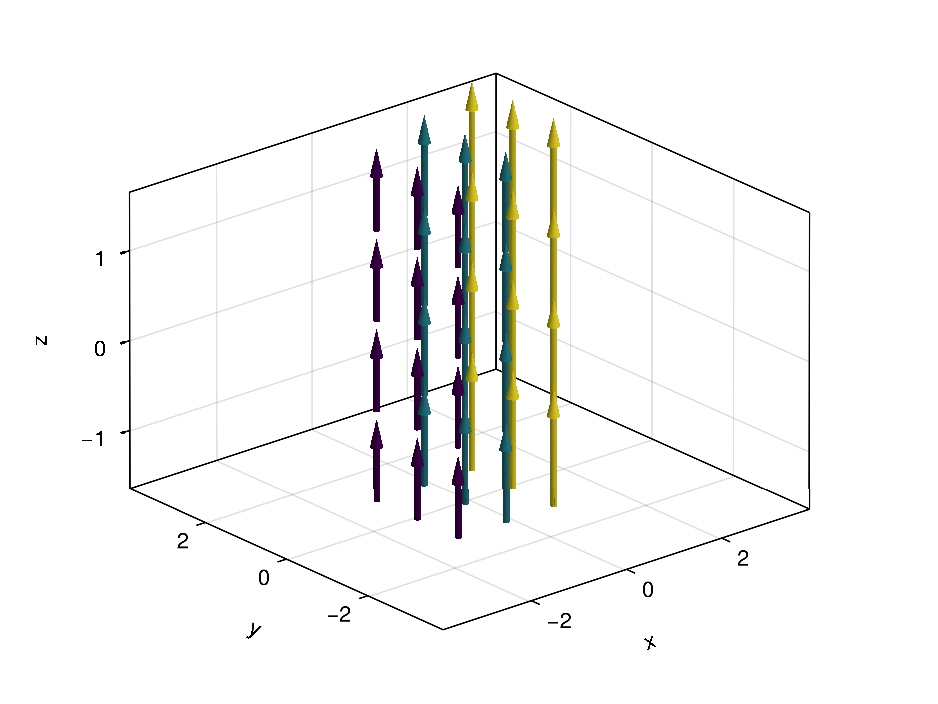
\includegraphics[width=\textwidth]{../figures/homo-cdp-j-field.pdf}
      \caption{Exemplary uniform, homogeneous current density vector field $\vec{j}(\vec{x}) = {j}_0 (-1, -1, 2)^T \mathds{1}_{\vec{x} \in \Omega_s}$ on a sample rectangular domain.}
      \label{fig:demo-cdp-j-field}
    \end{subfigure}
    \hfill
    \begin{subfigure}[t]{0.48\textwidth}
      \centering
      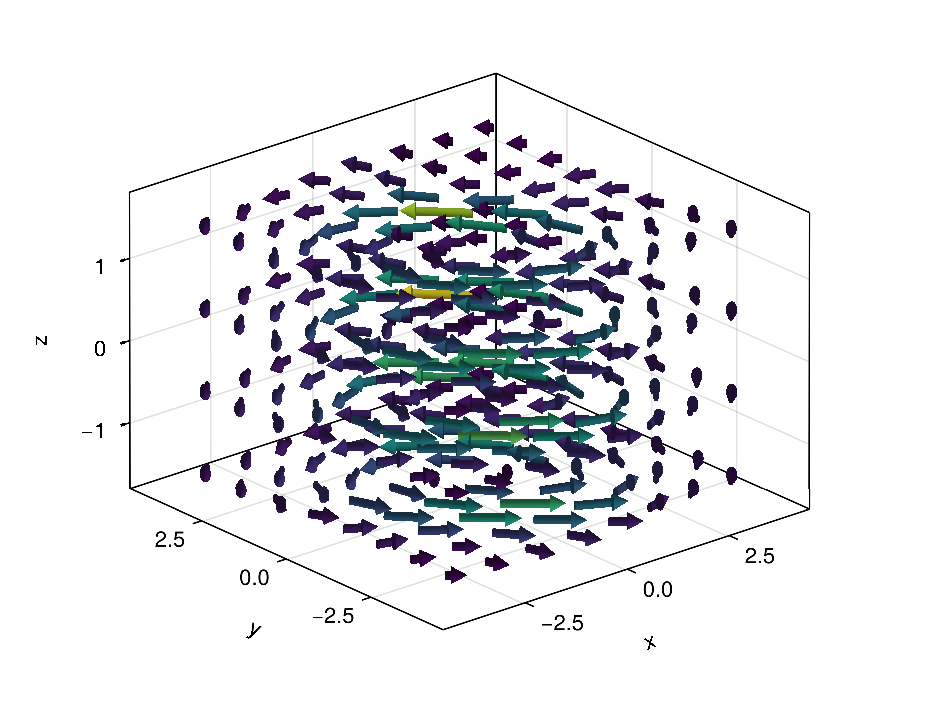
\includegraphics[width=\textwidth]{../figures/homo-cdp-b-field.pdf}
      \caption{Magnetic field $\vec{B}(\vec{x})$ resulting from the homogeneous current density field depicted in \Cref{fig:demo-cdp-j-field}.}
      \label{fig:demo-cdp-b-field}
    \end{subfigure}
    \caption{Current density field $\vec{j}$ and the corresponding magnetic field $\vec{B}$ as obtained using the Biot-Savart law.}
  \end{figure}

  \subsubsection{Gridded Data Format}
  In order to use KomaMRI together with the \gls{fft}-based evaluation of the Biot-Savart law on a phantom, we had to adapt the storage format from Koma's flattened vector storage of coordinates, density and other characteristic constants to a grid-based approach.
  The flattened storage format allows for higher efficiency in terms of memory usage, especially for less dense phantoms.
  However, some calculations on the data require neighbouring spins' characteristics in all six directions, for which a three-dimensional tensor storage format is more suitable, as it is provided in, for example, the JEMRIS file format (arrays are stored in \texttt{.h5} files).
  This is especially true for the FFT, where data must be provided in gridded format.

  \subsection{The Optimisation Approach}
  \label{sec:optimisation-procedure}
  In order to be able to reconstruct the current density vector field $\vec{j}$ and conductivity scalar field $\sigma$, we employed the following optimisation model:
  \begin{align*}
    \vec{B}^*, \sigma^* & = \argmin_{\vec{B}, \sigma} &  & \frac{1}{2} \int_\Omega \norm{\{\vec{B}\}_3 - B_3^0}^2 \,\dd\vec{x} + \frac{\alpha}{2} \int_\Omega \frac{\norm{\nabla \times \vec{B}(\vec{x})}^2}{\sigma(\vec{x})} \idd\vec{x} + R(\sigma) \\
                        & \text{subject to}           &  & \nabla \cdot \vec{B} = \div \vec{B} = 0                                                                                                                                                    \\
                        & \text{and}                  &  & \sigma \in [\sigma_0, \sigma_1]
  \end{align*}

  One may include the constraint as a penalty term to the objective function:
  \begin{align*}
    \int_\Omega \norm{\div \vec{B}(\vec{x})} \idd\vec{x} & = \int_\Omega \sqrt{\left(\frac{\partial B_1}{\partial x_1}\right)^2 + \left(\frac{\partial B_2}{\partial x_2}\right)^2 + \left(\frac{\partial B_3}{\partial x_3}\right)^2} \,\ddx_1\ddx_2\ddx_3    \\
                                                         & \leq \int_\Omega \left(\left|\frac{\partial B_1}{\partial x_1}\right| + \left|\frac{\partial B_2}{\partial x_2}\right| + \left|\frac{\partial B_3}{\partial x_3}\right|\right) \,\ddx_1\ddx_2\ddx_3
  \end{align*}

  Even better, we square
  \begin{align*}
    p_{\rm div} & = \int_\Omega \norm{\div \vec{B}(\vec{x})}^2 \idd\vec{x} = \int_{\Omega} \norm{\nabla \cdot \vec{B}(x_1, x_2, x_3)}^2 \,\ddx_1\ddx_2\ddx_3                                                             \\
                & = \int_\Omega \left(\left(\frac{\partial B_1}{\partial x_1}\right)^2 + \left(\frac{\partial B_2}{\partial x_2}\right)^2 + \left(\frac{\partial B_3}{\partial x_3}\right)^2\right) \,\ddx_1\ddx_2\ddx_3
  \end{align*}

  As a regulariser for the conductivity $\sigma$, we used the \gls{tv}, 1-norm of the gradient, of $\sigma$.

  Using Maxwell's second equation, one can obtain the corresponding current density $\vec{j}^*$ from Maxwell's fourth equation in the electrostatic case (\Cref{eq:maxwell-4-electrostatic}),
  $$\vec{j}^* = \frac{1}{\mu_0} (\nabla \times \vec{B}^*) = \frac{1}{\mu_0} \curl(\vec{B}^*)\,,$$
  where we evaluated the $\curl$ using a central finite difference scheme (setting boundary values to 0).

  \paragraph{Dimensional Analysis}
  Note the unit of the integral kernel: the numerator is the squared norm of the current density, therefore in \unit{\ampere\squared\per\meter^4}. Together with the corresponding denominator (\unit{\siemens\per\meter}), the integral kernel has units of \unit{\ampere\squared\ohm\per\meter^3}, becoming \unit{\ampere\squared\ohm}, which can be simplified to \unit{\volt\ampere}, which is a unit of \textbf{power} (\unit{\volt\ampere} = \unit{W}).
  This may be interpreted as a form of power dissipation outside of the domain and should therefore be minimised.

  The iterates were produced using the Optim.jl optimisation library \parencite{2018-optim-jl} using the LBFGS routine \parencite{1989-lbfgs}.

  \section{Results}
  \label{sec:results}
  Starting from an exemplary current density phantom (cf. \Cref{fig:cdpr-j-field}), the reconstruction routine converges after 40 LBFGS iterations, taking \SI{20}{\second} in total.
  The reconstructed current density may be found to its right, in \Cref{fig:cdprr-j-field}.
  The corresponding reconstructed conductivity and magnetic field, along with their originals can be found in \Cref{fig:sigma,fig:b-field}.

  \begin{figure}[H]
    \centering
    \begin{subfigure}[t]{0.48\textwidth}
      \centering
      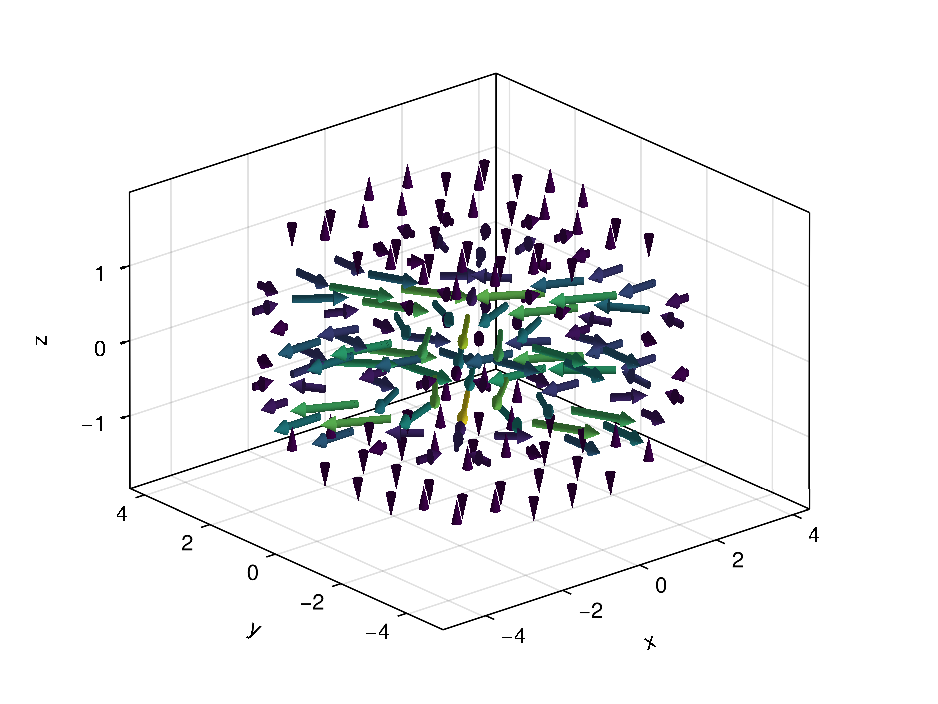
\includegraphics[width=\textwidth]{../figures/cdpr-j-field.pdf}
      \caption{Exemplary current density field $\vec{j}(\vec{x})$ on a sample rectangular domain.}
      \label{fig:cdpr-j-field}
    \end{subfigure}
    \hfill
    \begin{subfigure}[t]{0.48\textwidth}
      \centering
      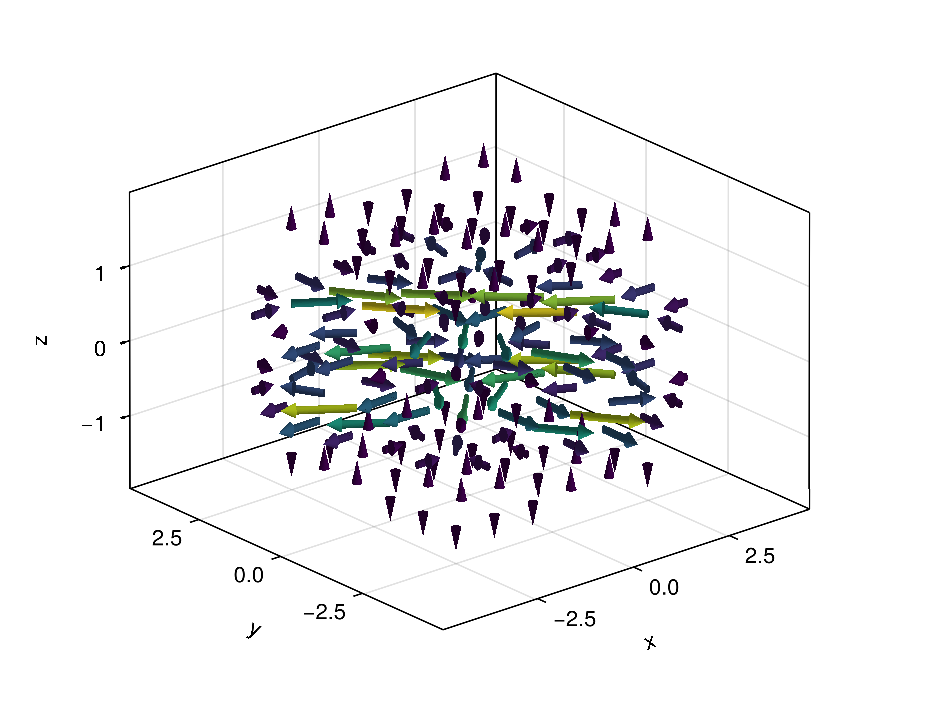
\includegraphics[width=\textwidth]{../figures/cdprr-j-field.pdf}
      \caption{The \textit{reconstructed} current density field $\vec{j}^*(\vec{x})$ using the method described in \Cref{sec:optimisation-procedure}.}
      \label{fig:cdprr-j-field}
    \end{subfigure}
    \caption{Original current density field $\vec{j}$ (left) and its reconstruction $\vec{j}^*$ (right).}
    \label{fig:j-field}
  \end{figure}

  \begin{figure}[H]
    \centering
    \begin{subfigure}[t]{0.48\textwidth}
      \centering
      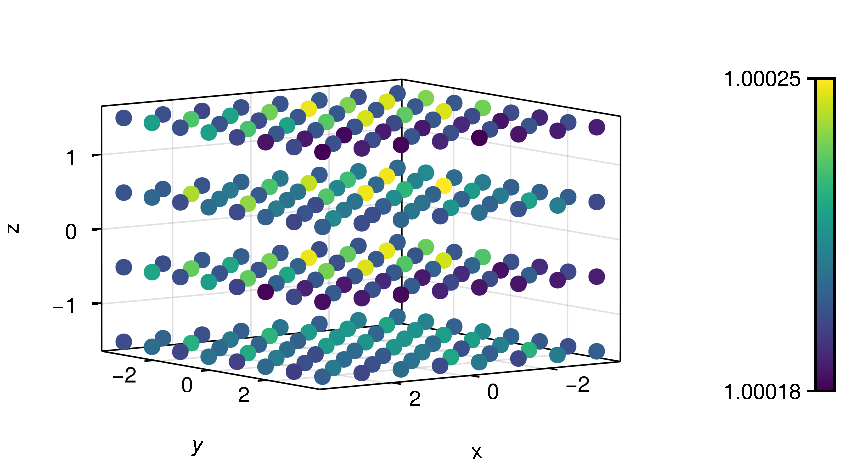
\includegraphics[width=\textwidth]{../figures/cdpr-sigma.pdf}
      \caption{Conductivity $\sigma$ of the original, obtained as the best possible combination with $\vec{j}$ and $\vec{B}$ using the optimisation described in \Cref{sec:optimisation-procedure}.}
      \label{fig:cdpr-sigma}
    \end{subfigure}
    \hfill
    \begin{subfigure}[t]{0.48\textwidth}
      \centering
      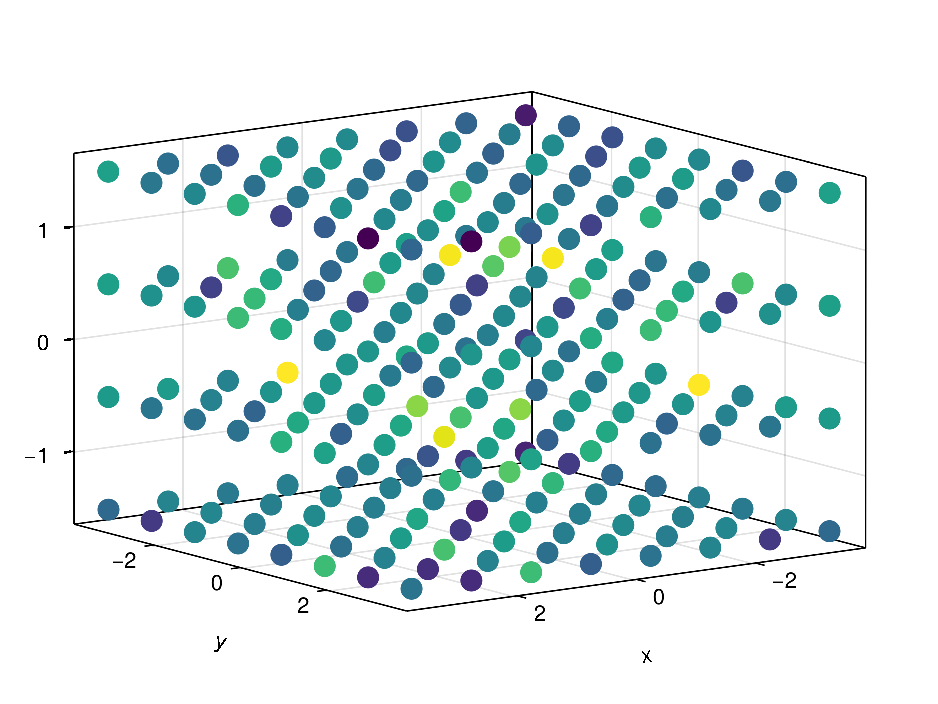
\includegraphics[width=\textwidth]{../figures/cdprr-sigma.pdf}
      \caption{Reconstructed conductivity field $\sigma$, marking the solution of the optimisation problem together with \Cref{fig:cdprr-j-field,fig:cdprr-b-field}.}
      \label{fig:cdprr-sigma}
    \end{subfigure}
    \caption{Original conductivity $\sigma$ (left) and its reconstruction $\sigma^*$ (right).}
    \label{fig:sigma}
  \end{figure}

  \begin{figure}[H]
    \centering
    \begin{subfigure}[t]{0.48\textwidth}
      \centering
      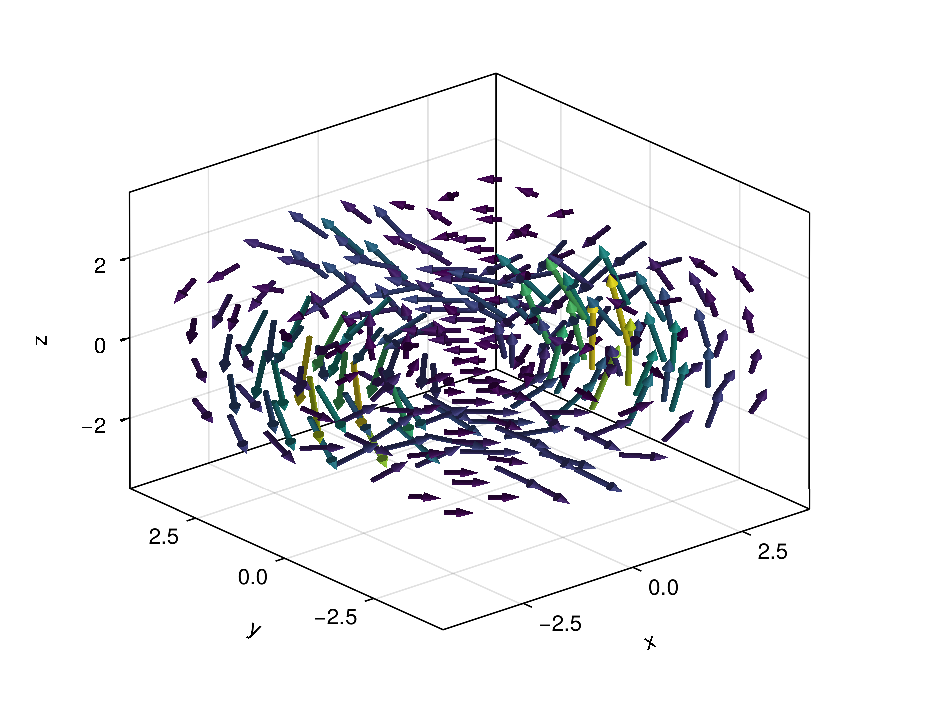
\includegraphics[width=\textwidth]{../figures/cdpr-b-field.pdf}
      \caption{Magnetic field corresponding to the current density field in \Cref{fig:cdpr-j-field}, as obtained through the Biot-Savart law.}
      \label{fig:cdpr-b-field}
    \end{subfigure}
    \hfill
    \begin{subfigure}[t]{0.48\textwidth}
      \centering
      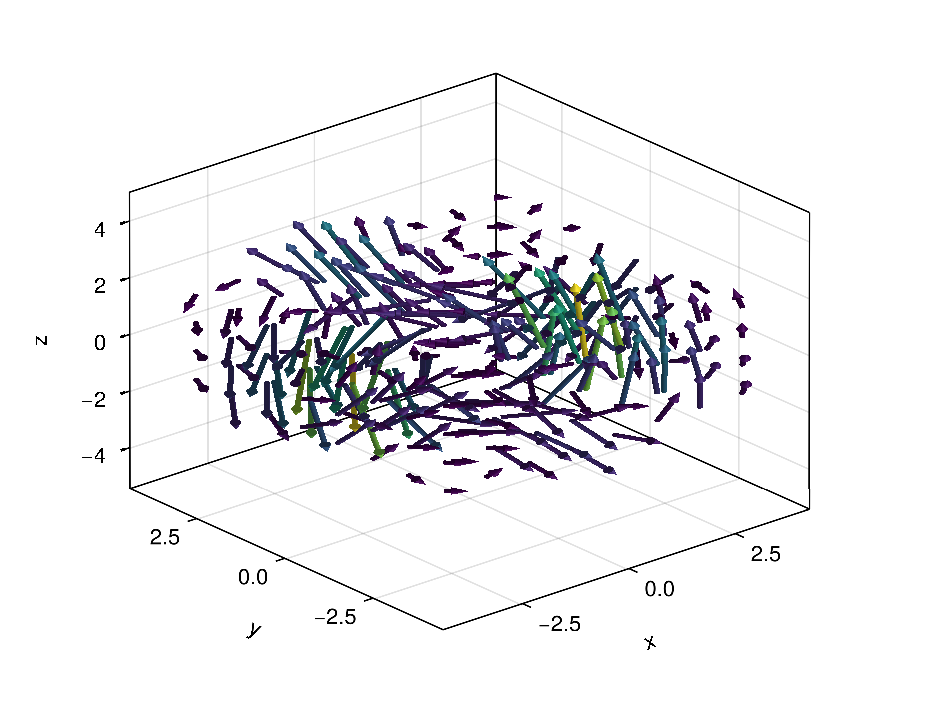
\includegraphics[width=\textwidth]{../figures/cdprr-b-field.pdf}
      \caption{Magnetic field corresponding to the \textit{reconstructed} current density \Cref{fig:cdprr-j-field}, as obtained through the Biot-Savart law.}
      \label{fig:cdprr-b-field}
    \end{subfigure}
    \caption{Original magnetic field $\vec{B}$ (left) and its reconstruction $\vec{B}^*$ (right).}
    \label{fig:b-field}
  \end{figure}

  \subsection{Usage as a Julia Package}
  The package provides two abstractions of Koma's \texttt{phantom} class:
  \begin{enumerate}
    \item \texttt{PhantomOnAGrid}, implementing the conversion and interfacing to the gridded data format.
    \item \texttt{CurrentDensityPhantom}, extending \texttt{PhantomOnAGrid} with the current density vector field (each spatial component is stored in its own respective tensor).
  \end{enumerate}

  In order to install and try out the package, open up a Julia live interpreter and type:
  \begin{minted}{julia}
    import Pkg; Pkg.add(url="https://github.com/MrP01/CurrentDensityImaging");
    import CurrentDensityImaging as CDI  # import the package
    cdp = CDI.generateDemoCDP()  # generate exemplary current density phantom
  \end{minted}

  With the constructed current density phantom (\texttt{cdp}), one can generate plots for $\vec{j}$, $\vec{B}$ and $\sigma$ using
  \texttt{CDI.plot\_current\_density},
  \texttt{CDI.plot\_magnetic\_field} and
  \texttt{CDI.plot\_conductivity}, respectively.
  It is also possible to load a phantom in the JEMRIS format, for more information we refer the reader to the \href{https://github.com/MrP01/CurrentDensityImaging}{code repository}.

  The forward operator (FFT-accelerated evaluation of the Biot-Savart equation) can be invoked as follows:
  \begin{minted}{julia}
    B1, B2, B3 = CDI.calculate_magnetic_field(cdp);  # obtain the x, y and z components of B
  \end{minted}

  A reconstruction from the z-component of the magnetic field $B_z$ can be obtained using
  \begin{minted}{julia}
    cdpr, sigmar = CDI.solve(B3);  # reconstruction of j and sigma
  \end{minted}
  where \texttt{cdpr} contains the reconstructed current density phantom and $\sigma$\texttt{r} is the reconstructed conductivity.

  \section{Future Perspectives}
  \gls{mrcdi} is a promising approach toward the better diagnosis of pathologies in patients using imaging techniques.
  The given model can be extended in various ways, for example one could modify the regularisation imposed on the conductivity, or add further terms to generally improve the reconstruction of $\vec{j}$.
  It might also be possible to relax the divergence freeness condition in the optimisation procedure, by reducing redundancy in the optimised variable space.

  As suggested by Prof. Bredies, one could approach the problem using an alternative model and optimisation routine, given in \Cref{sec:alt-formulation}.

  \section*{Signatures}

  \vspace{4cm}
  \SignatureAndDate{(Peter Waldert)}

  \vspace{3cm}
  \SignatureAndDate{(Prof. Kristian Bredies)}

  \pagebreak
  \printbibliography
  \printnoidxglossary[type=acronym, title={Acronyms}]

  \pagebreak
  \appendix
  \section{Appendix}
  The figures in this report were generated using Makie \parencite{2021-makie}.

  \subsection{Alternate Formulation and Splitting Method}
  \label{sec:alt-formulation}
  \begin{align*}
    \vec{B}^*, \sigma^* & = \argmin_{\vec{B}, \sigma}
  \end{align*}

  \begin{figure}[H]
    \centering
    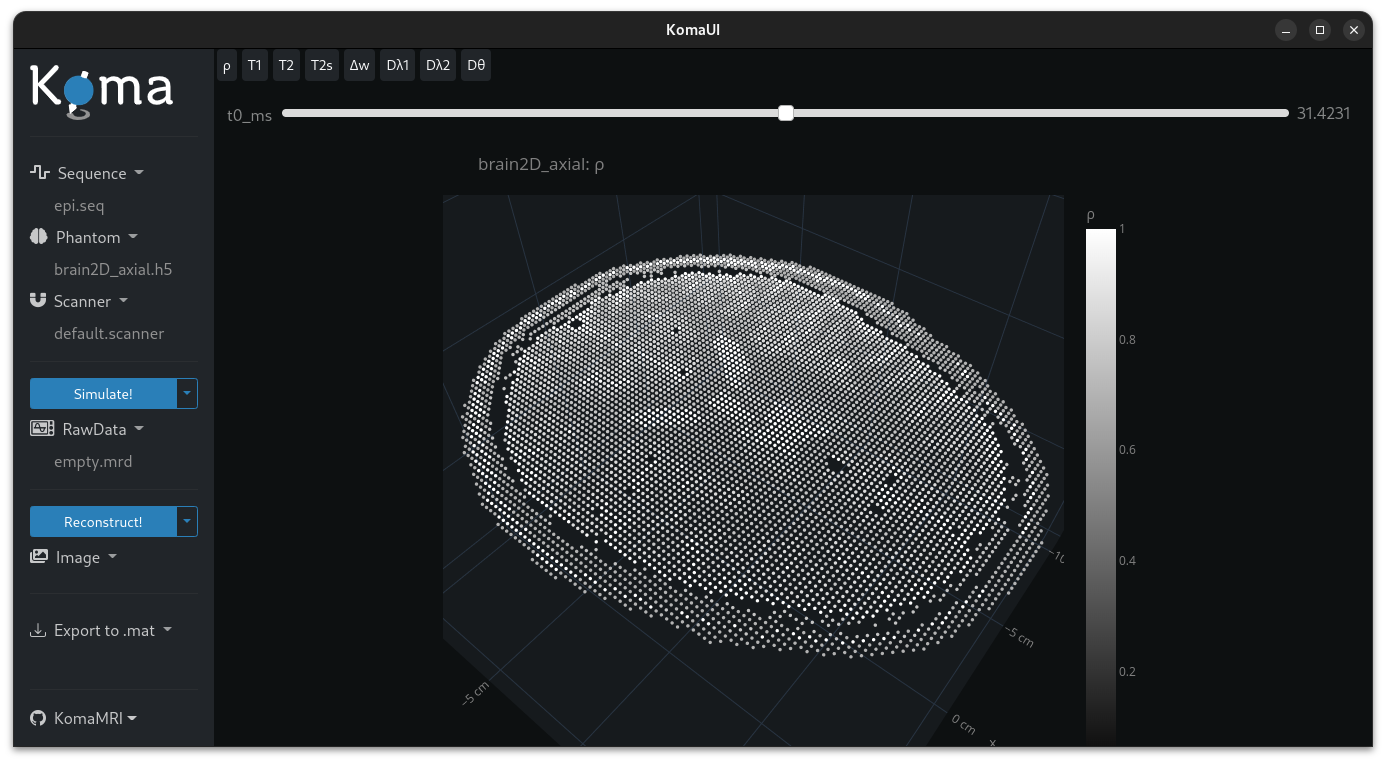
\includegraphics[width=\linewidth]{../figures/komaui.png}
    \caption{Koma UI}
    \label{fig:komaui}
  \end{figure}

  \begin{figure}[H]
    \begin{subfigure}[t]{0.48\textwidth}
      \centering
      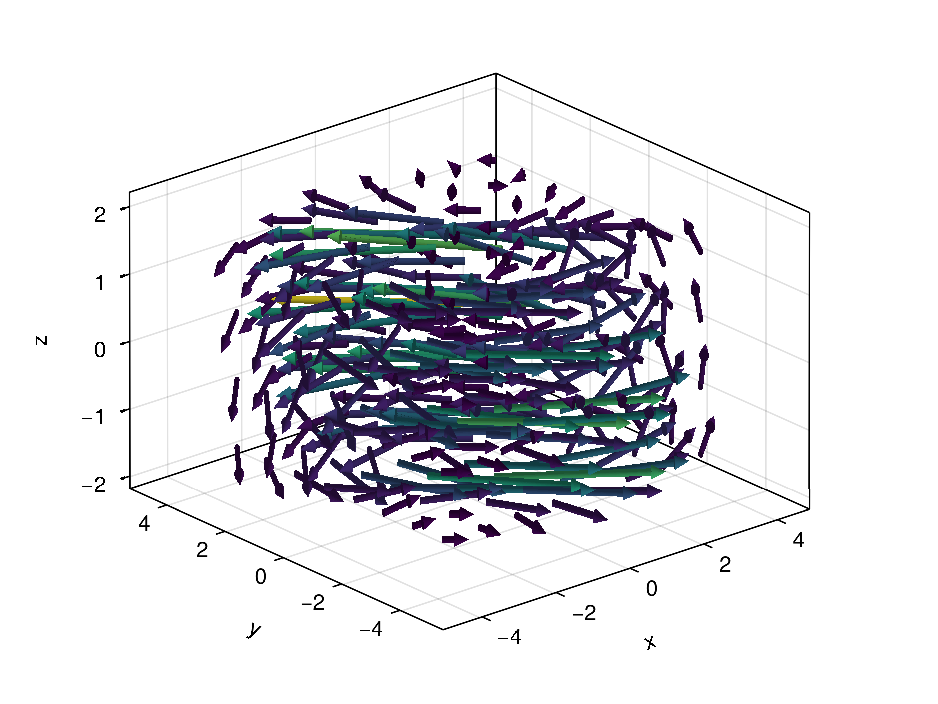
\includegraphics[width=\textwidth]{../figures/cdpbr-b-field.pdf}
      \caption{Magnetic field obtained from the Biot-Savart procedure of the $\curl$ of the $\vec{B}$-field in \Cref{fig:demo-cdp-b-field}.}
      \label{fig:cdpbr-b-field}
    \end{subfigure}
  \end{figure}
\end{document}
